Idea behind compact mappings, and why it does not work. Basically:\cite{goens_samos19}


\begin{figure*}[th]
	\centering
	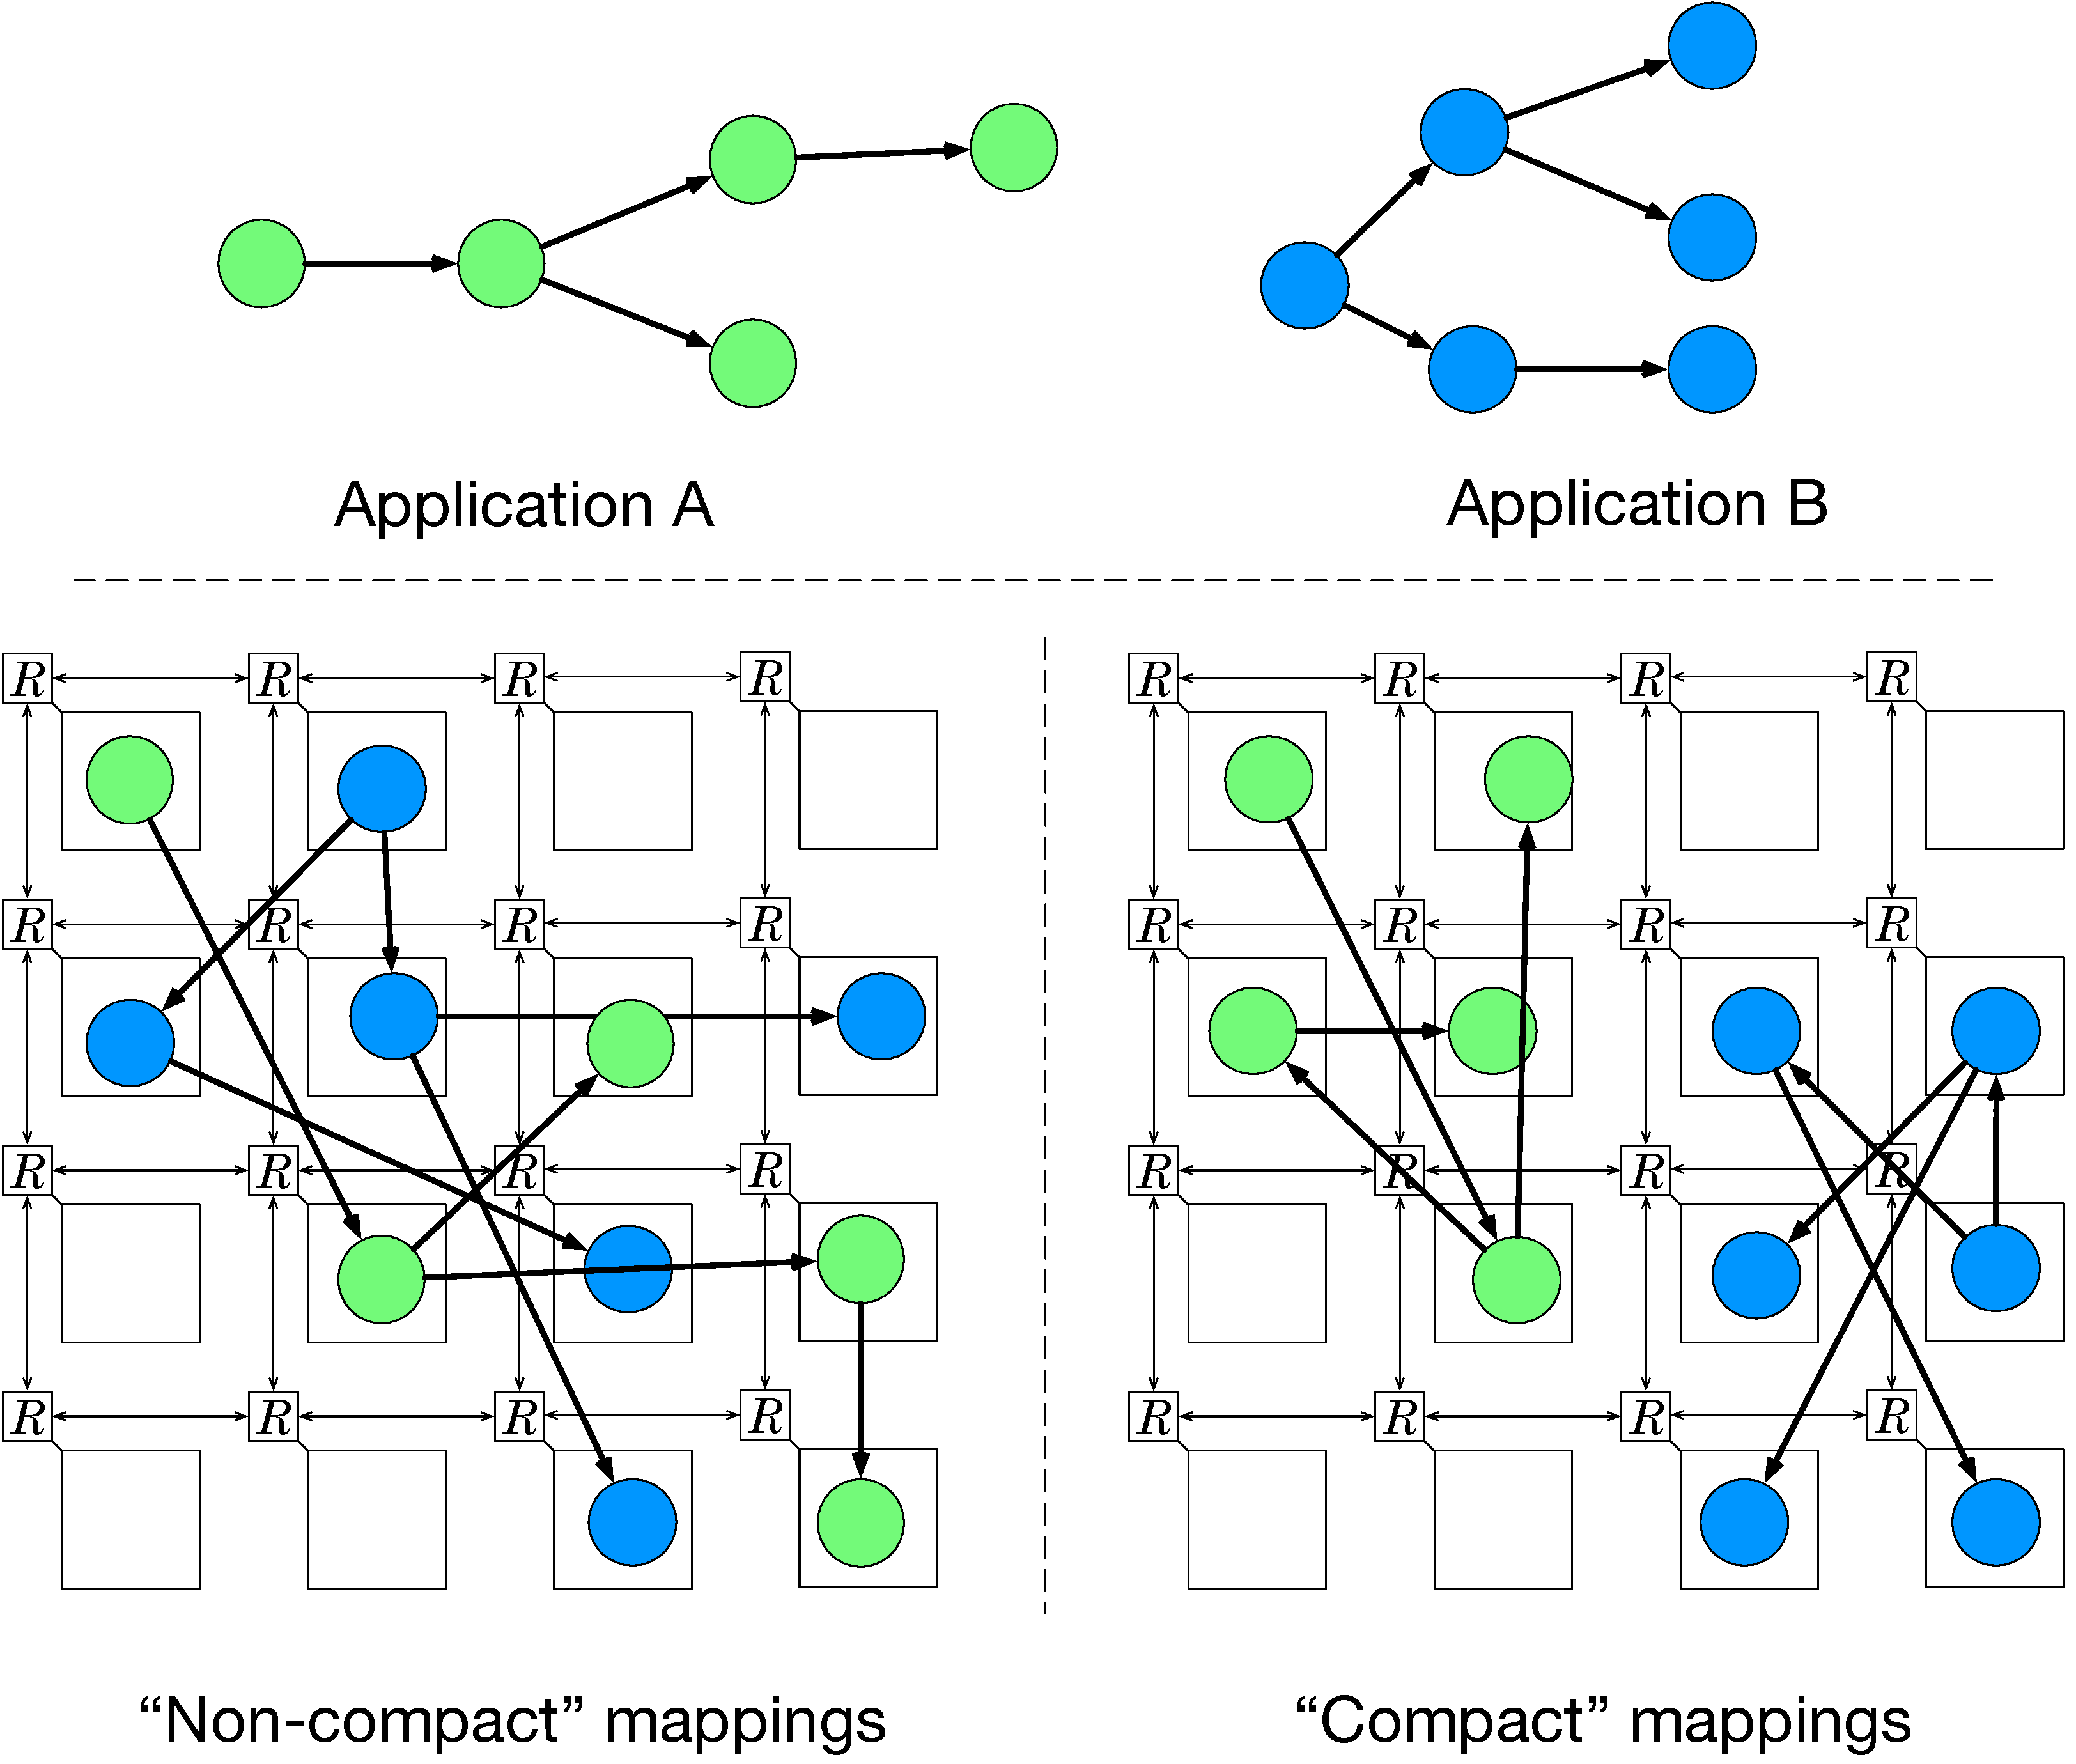
\includegraphics[width=0.6\textwidth]{figures/compact_intro.pdf}
	\caption{Equivalent mappings of two applications, one being compact and the other one not. Adapted from Figure~1 in~\cite{goens_samos19}.}
	\label{fig:compact_intro}
\end{figure*}


\begin{figure*}[th]
	\centering
	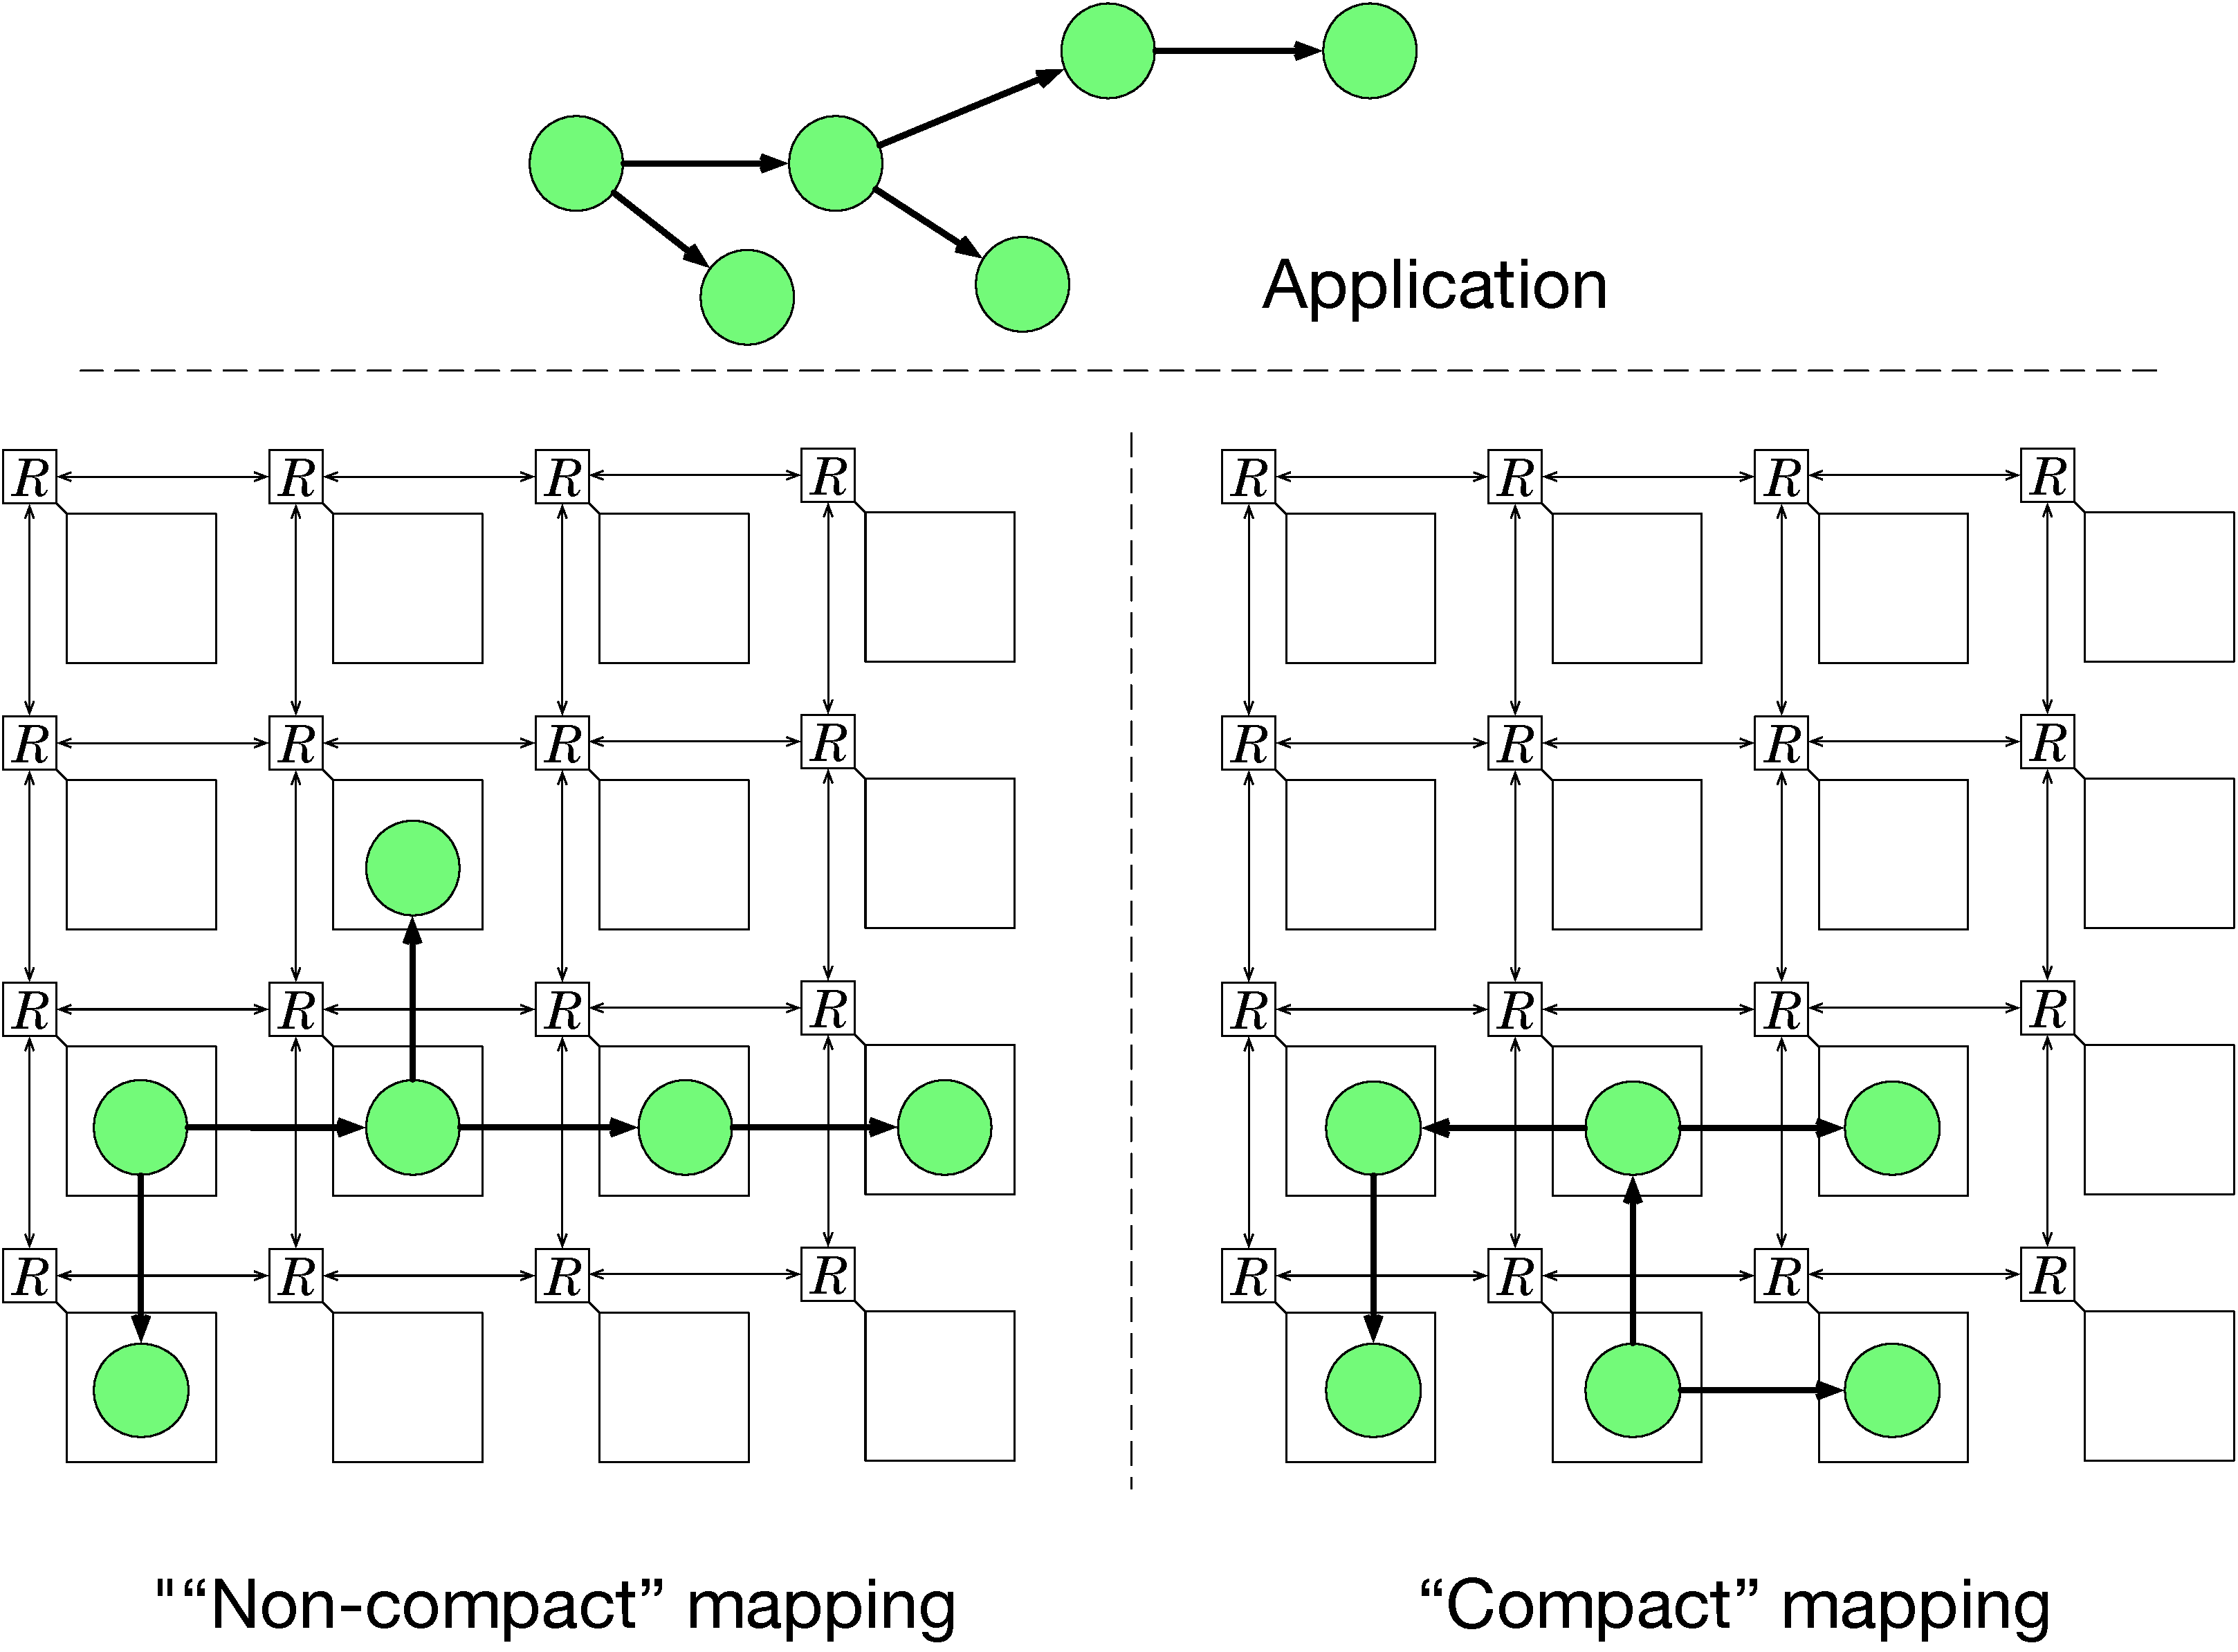
\includegraphics[width=0.6\textwidth]{figures/topology_vs_geometry.pdf}
	\caption{Two equivalent mappings that yield good performance. Adapted from Figure~2 in~\cite{goens_samos19}.}
	\label{fig:topology_vs_geometry}
\end{figure*}


\begin{figure}[h]
	\centering
   \resizebox{0.85\textwidth}{!}{\inputTikz{compact_latency.tex}}
	\caption{Comparison of latencies between compact, non-compact and random mappings. Adapted from Figure~4 in~\cite{goens_samos19}.}
	\label{fig:compact_latency}
\end{figure}


\begin{figure}[h]
	\centering
   \resizebox{0.85\textwidth}{!}{\inputTikz{compact_cases.tex}}
	\caption{Comparison between compact, non-compact and random mappings running isolation or with another 9 applications. Adapted from Figure~5 in~\cite{goens_samos19}.}
	\label{fig:compact_cases}
\end{figure}